\clearpage
\myparagraph{First \olly example: a=1.2 and b=3.4}
\myindex{\olly}

Both \FLD are executed:

\begin{figure}[H]
\centering
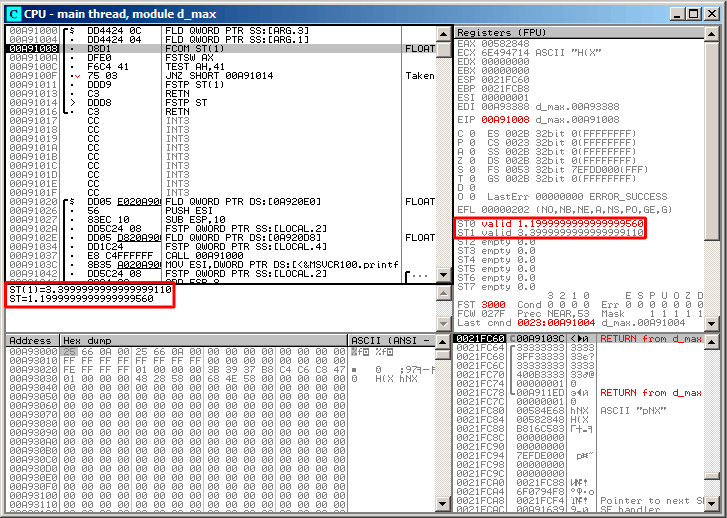
\includegraphics[scale=\FigScale]{patterns/12_FPU/3_comparison/x86/MSVC_Ox/olly1_1.png}
\caption{\olly: both \FLD are executed}
\label{fig:FPU_comparison_Ox_case1_olly1}
\end{figure}

\FCOM being executed: 
\olly shows the contents of \ST{0} and \ST{1} %
for convenience.

\clearpage
\FCOM is done:

\begin{figure}[H]
\centering
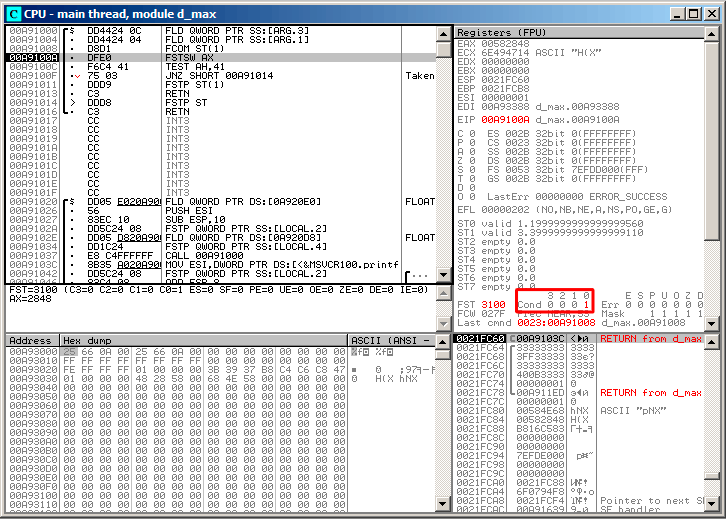
\includegraphics[scale=\FigScale]{patterns/12_FPU/3_comparison/x86/MSVC_Ox/olly1_2.png}
\caption{\olly: \FCOM is done}
\label{fig:FPU_comparison_Ox_case1_olly2}
\end{figure}

\Czero is set, all other condition flags are cleared.

\clearpage
\FNSTSW is done, \GTT{AX}=0x3100:

\begin{figure}[H]
\centering
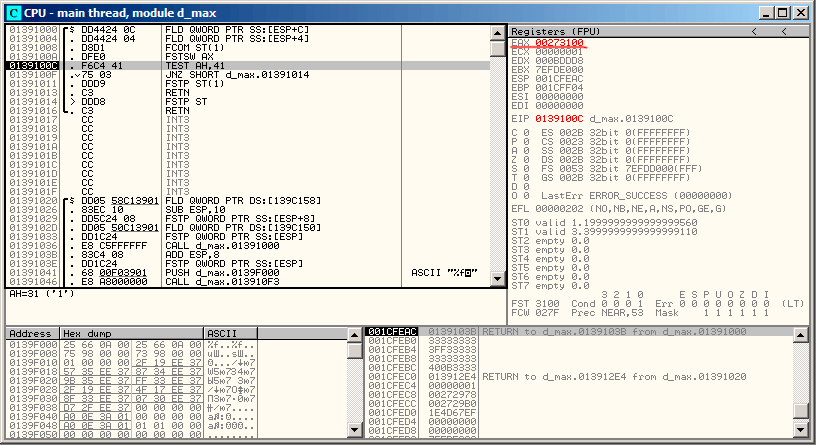
\includegraphics[scale=\FigScale]{patterns/12_FPU/3_comparison/x86/MSVC_Ox/olly1_3.png}
\caption{\olly: \FNSTSW is executed}
\label{fig:FPU_comparison_Ox_case1_olly3}
\end{figure}

\clearpage
\TEST is executed:

\begin{figure}[H]
\centering
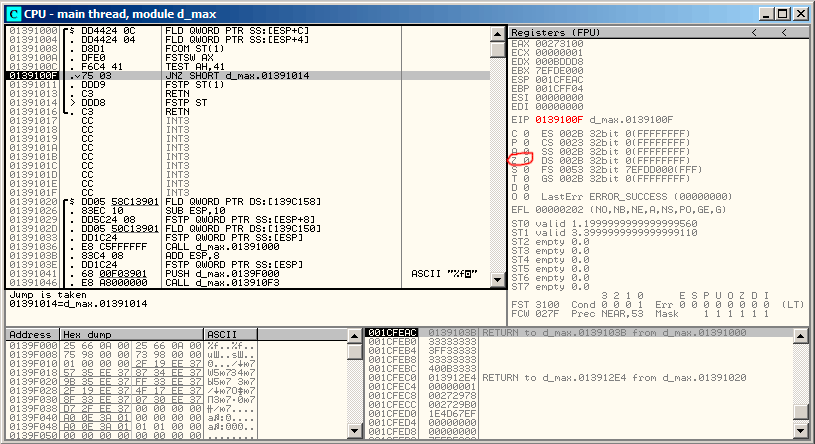
\includegraphics[scale=\FigScale]{patterns/12_FPU/3_comparison/x86/MSVC_Ox/olly1_4.png}
\caption{\olly: \TEST is executed}
\label{fig:FPU_comparison_Ox_case1_olly4}
\end{figure}

ZF=0, conditional jump is about to trigger now.

\clearpage
\INS{FSTP ST} (or \FSTP \ST{0}) was executed~---1.2 was popped from the stack, and 3.4 was left on top:

\begin{figure}[H]
\centering
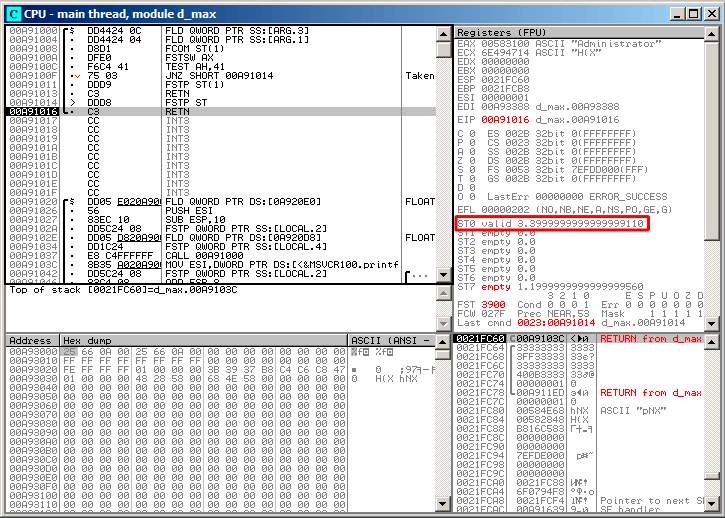
\includegraphics[scale=\FigScale]{patterns/12_FPU/3_comparison/x86/MSVC_Ox/olly1_5.png}
\caption{\olly: \FSTP is executed}
\label{fig:FPU_comparison_Ox_case1_olly5}
\end{figure}

We see that the \INS{FSTP ST} 

instruction works just like popping one value from the FPU stack.

\clearpage
\myparagraph{Second \olly example: a=5.6 and b=-4}

Both \FLD are executed:

\begin{figure}[H]
\centering
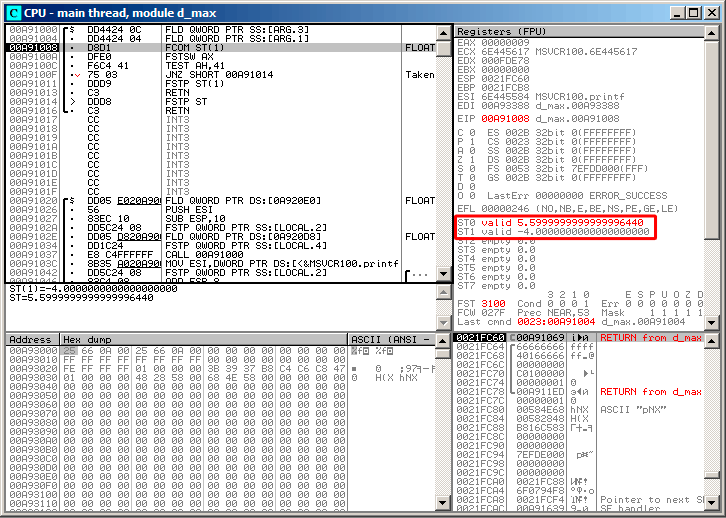
\includegraphics[scale=\FigScale]{patterns/12_FPU/3_comparison/x86/MSVC_Ox/olly2_1.png}
\caption{\olly: both \FLD are executed}
\label{fig:FPU_comparison_Ox_case2_olly1}
\end{figure}

\FCOM is about to execute.

\clearpage
\FCOM is done:

\begin{figure}[H]
\centering
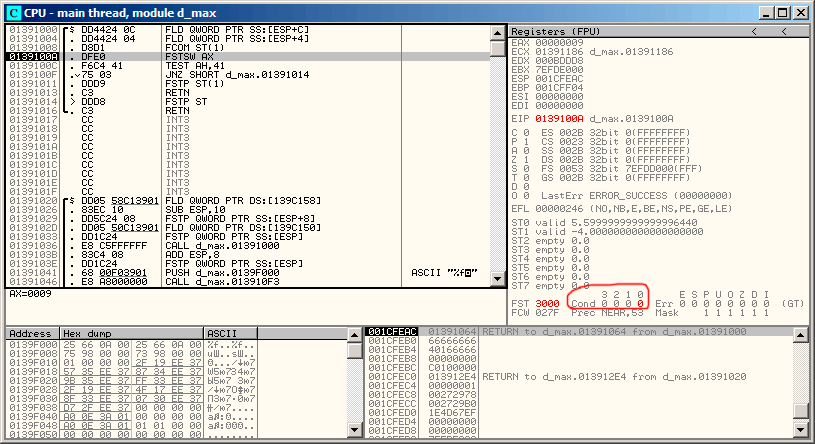
\includegraphics[scale=\FigScale]{patterns/12_FPU/3_comparison/x86/MSVC_Ox/olly2_2.png}
\caption{\olly: \FCOM is finished}
\label{fig:FPU_comparison_Ox_case2_olly2}
\end{figure}

All conditional flags are cleared.

\clearpage
\FNSTSW done, \GTT{AX}=0x3000:

\begin{figure}[H]
\centering
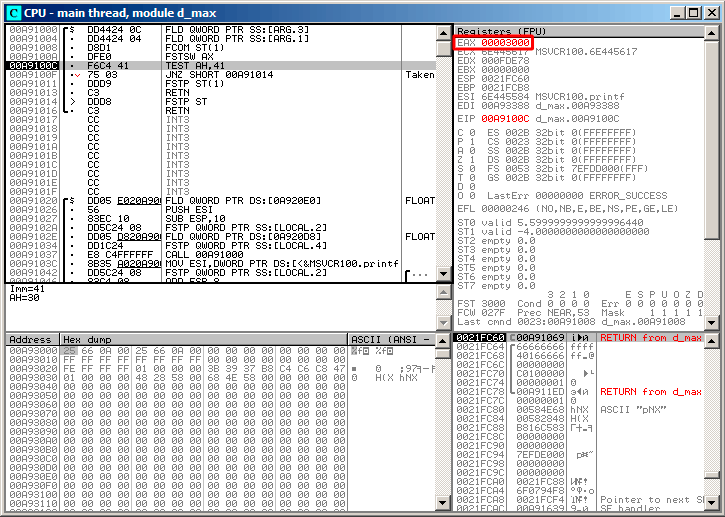
\includegraphics[scale=\FigScale]{patterns/12_FPU/3_comparison/x86/MSVC_Ox/olly2_3.png}
\caption{\olly: \FNSTSW was executed}
\label{fig:FPU_comparison_Ox_case2_olly3}
\end{figure}

\clearpage
\TEST is done:

\begin{figure}[H]
\centering
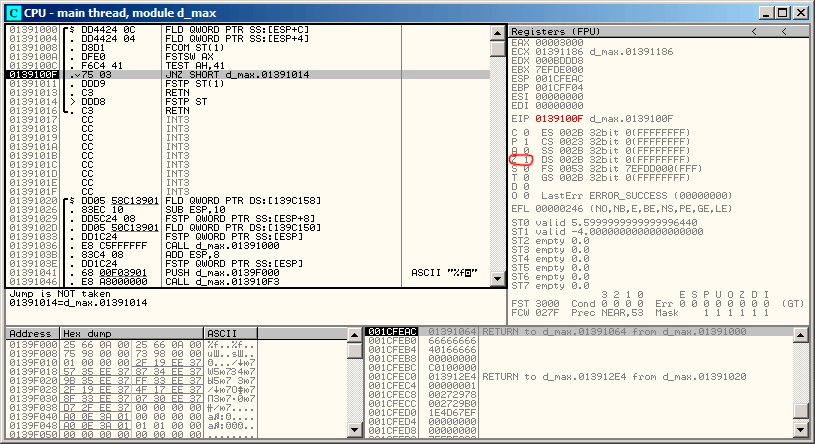
\includegraphics[scale=\FigScale]{patterns/12_FPU/3_comparison/x86/MSVC_Ox/olly2_4.png}
\caption{\olly: \TEST was executed}
\label{fig:FPU_comparison_Ox_case2_olly4}
\end{figure}

ZF=1, jump will not happen now.

\clearpage
\FSTP \ST{1} was executed: a value of 5.6 is now at the top of the FPU stack.

\begin{figure}[H]
\centering
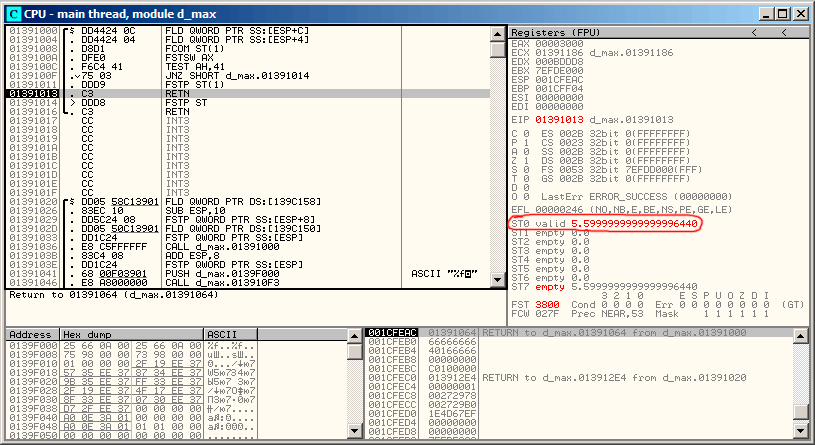
\includegraphics[scale=\FigScale]{patterns/12_FPU/3_comparison/x86/MSVC_Ox/olly2_5.png}
\caption{\olly: \FSTP was executed}
\label{fig:FPU_comparison_Ox_case2_olly5}
\end{figure}

We now see that the \FSTP \ST{1} 

instruction works as follows: it leaves what was at the top of the stack, but clears \ST{1}.

